\documentclass[letterpaper,twocolumn,openany]{dndbook}

\usepackage[english]{babel}
\usepackage[utf8]{inputenc}
\usepackage[singlelinecheck=false]{caption}
\usepackage{lipsum}
\usepackage{listings}
\usepackage{shortvrb}
\usepackage{imakeidx}
\usepackage[open,openlevel=1]{bookmark}

\usepackage[table]{xcolor}
\usepackage{everypage}
\usepackage{calc}
\usepackage[absolute]{textpos}
\usepackage{lettrine}
\usepackage{lipsum}
\usepackage{environ}
\usepackage{multirow,makecell}
\usepackage{dblfloatfix}
\usepackage{multicol}
\usepackage{overpic}
\usepackage{changepage}
\usepackage{luatexja}
\usepackage{xcolor}
\usepackage{pdfrender}
\usepackage{fontspec}
\usepackage{tikz}
\usepackage[export]{adjustbox}
\usepackage{luatexja-fontspec}
\usepackage{supertabular}
\usepackage[titles]{tocloft}
\usepackage[titletoc]{appendix}
\usepackage{biblatex}
\usepackage{microtype}
\usepackage{csquotes}
\usepackage{xpatch}

\MakeShortVerb{|}

\lstset{%
	basicstyle=\ttfamily,
	language=[LaTeX]{TeX},
	breaklines=true,
}

\definecolor{CharFillColor}{rgb}{1,1,1}

\captionsetup[table]{labelformat=empty,font={sf,sc,bf,},skip=0pt}

% Remove reference numbers from Inspiration/Bibliography
\DeclareFieldFormat{labelnumberwidth}{}
\setlength{\biblabelsep}{0pt}

%!TEX TS-program = xelatex
%!TEX encoding = UTF-8 Unicode

% Author: Romain "Artefact2" Dal Maso <artefact2@gmail.com>
% 
% This program is free software. It comes without any warranty, to the
% extent permitted by applicable law. You can redistribute it and/or
% modify it under the terms of the Do What The Fuck You Want To Public
% License, Version 2, as published by Sam Hocevar. See
% http://sam.zoy.org/wtfpl/COPYING for more details.

\usepackage{AlegreyaSans}
\usepackage{tgbonum}

\newfontfamily\nodesto[
	Path = fonts/,
	Extension = .otf,
	UprightFont = *,
	BoldFont = * Bold,
	ItalicFont = * Italic,
	BoldItalicFont = * Bold Italic,
]{Nodesto Caps Condensed}

\newfontfamily\alegreyasansbold{Alegreya Sans Bold}
\newfontfamily\texgyrebonum{TeXGyreBonum-Bold}

\setmainfont{TeXGyreBonum}
\setsansfont{Alegreya Sans}
\setmainjfont{IPAexMincho}
\setsansjfont{IPAexGothic}

\newfontfamily\alegreyasans{Alegreya Sans}

\renewcommand{\gilliustwo}{\alegreyasans{}}
% Front cover page
\newcommand{\DndCoverSplotch}{img/cover-splotch}
\newcommand{\DndCoverSplotchText}{Splotch Text}
\newcommand{\DndSubcoverSubtitle}{Subcover Subtitle}
\newcommand{\DndTitle}{Cover Title}
\newcommand{\DndSubtitle}{Cover Subtitle}
\newcommand{\DndTagline}{Cover Tagline}

\newlength\mylength
\renewcommand\cftchappresnum{\chaptername~}
\renewcommand\cftchapaftersnum{:}
\settowidth\mylength{\cftchappresnum\cftchapaftersnum\quad}
\addtolength\cftchapnumwidth{\mylength}

% StrokeColor, FillColor, StrokeWidth, Text
\newcommand*{\fillstroke}[4]{%
	% this is black magic
	% ref: http://tex.stackexchange.com/a/225639/125447
	% Tr: rendering mode (0=Fill, 1=Stroke, 2=FillThenStroke)
	% w: stroke width
	\special{pdf:bcolor #1 #2}%
	\special{pdf:literal direct #3 w 2 Tr}%
	#4%
	% ref: http://project.ktug.org/dvipdfmx/doc/tug2005.pdf
	\special{pdf:ecolor}%
	\special{pdf:literal direct 0 Tr}%
}

\newlength{\ox}
\newlength{\oy}

\ifdefined\isdraft
	\setlength{\ox}{.5\stockwidth-.5\paperwidth}
	\setlength{\oy}{.5\stockheight-.5\paperheight}
	\settrims{\oy}{\ox}
\else
	\setlength{\ox}{0pt}
	\setlength{\oy}{0pt}
\fi

\NewEnviron{tb*}[3]{%
	\begin{textblock*}{#1}(\ox+#2,\oy+#3)\BODY\end{textblock*}%
}

\NewEnviron{rtb*}[3]{%
	\TPoptions{absolute=false}%
	\begin{textblock*}{#1}(#2,#3)\BODY\end{textblock*}%
	\TPoptions{absolute=true}%
}

\newcommand*{\CoverPageBackground}[1]{
	\tikz[remember picture,overlay]
	\node[opacity=1,inner sep=0pt] at (current page.center)
	{
		\includegraphics[width=\paperwidth, keepaspectratio]{#1}
	};
}

\newcommand{\DndMakeCover}{
	\onecolumn%
	\thispagestyle{empty}%
	\CoverPageBackground{img/cover}
	\begin{center}%
		\vspace*{-15mm}
\includegraphics[width=3cm]{img/cover-logo-homebrewery}\\*\vspace*{15mm}%

		\fontsize{48pt}{48pt}\selectfont%
		\textpdfrender{
			TextRenderingMode=FillStroke,
			LineWidth=1.5pt,
			FillColor=CharFillColor,
		}{\nodesto{\DndTitle}}\\*%
		\normalfont\normalsize
\includegraphics[width=.5\paperwidth]{img/separator}\\%
		\fontsize{48pt}{48pt}\selectfont%
		%\textpdfrender{
		%	TextRenderingMode=FillStroke,
		%	LineWidth=1.5pt,
		%	FillColor=CharFillColor,
		%}{\DndSubtitle}\\*%
	\end{center}%
	\begin{figure*}[!b]
		\normalfont\normalsize
		\begin{adjustwidth}{-20mm}{0mm}
			\color{white}
			%\vspace*{17.0cm}
			\begin{overpic}[percent,unit=1mm,scale=.31]{\DndCoverSplotch}
				\put(12,5){\huge\texgyrebonum{\DndCoverSplotchText}}
			\end{overpic}
		\end{adjustwidth}
		\begin{center}%
			\normalfont\normalsize
			\LARGE\vfill%
			%https://tex.stackexchange.com/questions/25221/outlined-characters/108348#108348
			\textpdfrender{
				TextRenderingMode=FillStroke,
				LineWidth=0.5pt,
				FillColor=CharFillColor,
			}{\alegreyasansbold{\DndTagline}}\\*%
			% XXX: font doesn't look right
		\end{center}%
	\end{figure*}
	\pdfbookmark[0]{Front Cover}{Front Cover}
	\normalfont\normalsize
	\clearpage%
	\twocolumn%
}

\newcommand{\DndBlankPage}{%
	\onecolumn%
	\thispagestyle{empty}%
	\begin{center}%
		\LARGE\vfill%
	\end{center}%
	\normalfont\normalsize
	\clearpage%
	\twocolumn%
}

\newcommand{\DndMakeSubcover}{%
	\onecolumn%
	\thispagestyle{empty}%
	\begin{center}%
		\fontsize{48pt}{48pt}\selectfont%
		\nodesto{\bfseries{\DndTitle}}\\*%
		\normalfont\normalsize
\includegraphics[width=.5\paperwidth]{img/separator}\\%
		\fontsize{48pt}{48pt}\selectfont%
		%\DndSubtitle\\*%
		\normalfont\normalsize
		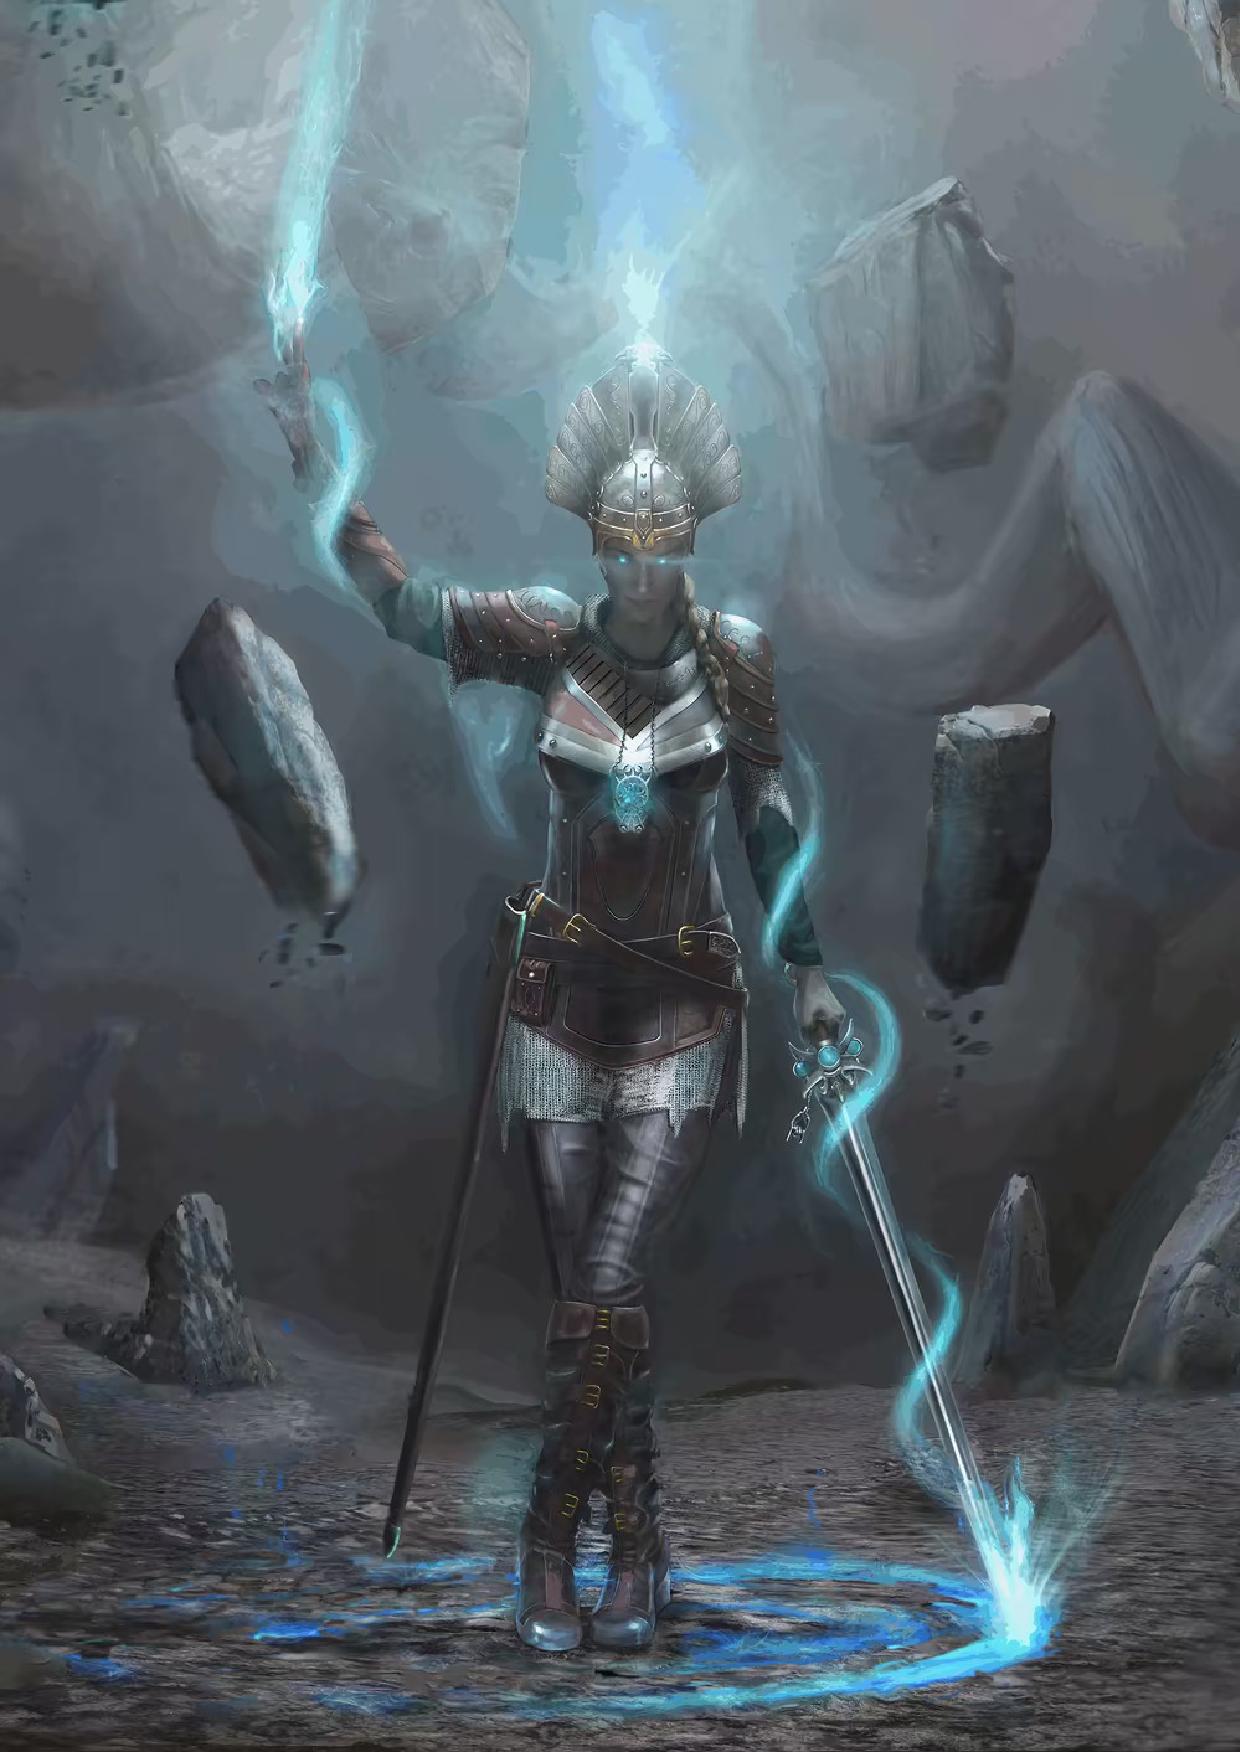
\includegraphics[width=10cm,keepaspectratio]{img/subcover}\\
		\LARGE\vfill%
		%\alegreyasansbold{\DndSubcoverSubtitle}\\%
		\vspace*{-15mm}
\includegraphics[width=3cm]{img/cover-logo-homebrewery}\\*\vspace*{15mm}%
	\end{center}%
	\normalfont\normalsize
	\clearpage%
	\twocolumn%
}

% Back cover page
\newcommand{\DndBackcover}{img/cover}
\newcommand{\DndBackcoverHeader}{Header.}
\newcommand{\DndBackcoverClose}{Closing sentence.}
\newcommand{\DndBackcoverDescription}{Description.}
\newcommand{\DndBackcoverLink}{\url{https://example.org}}
\newcommand{\DndBackcoverLogo}{img/dnd-logo-homebrewery}

\newcommand{\DndMakeBackcover}{%
	\onecolumn%
	\thispagestyle{empty}%
	\begin{tikzpicture}[remember picture,overlay]%
		\node[opacity=1, inner sep=0pt, anchor=east] (DndBackcover) at (current page.east)
		{
			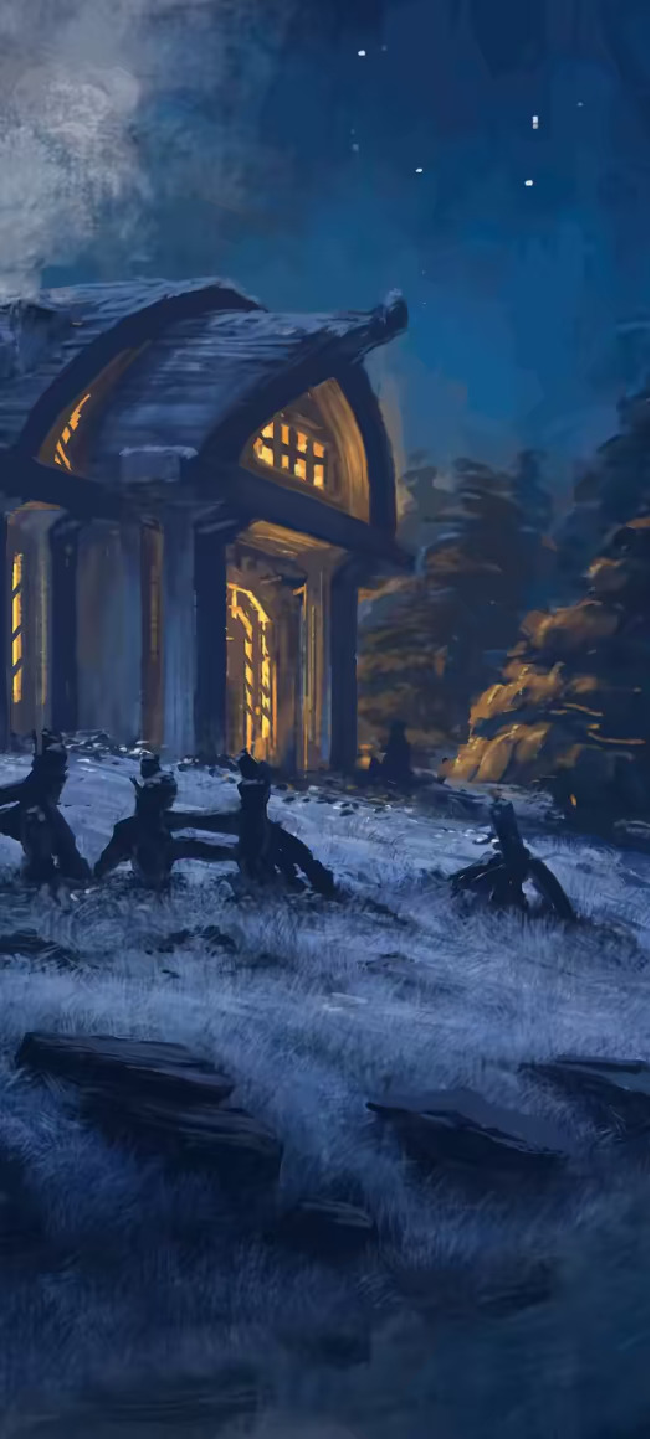
\includegraphics[width=\paperwidth,height=\paperheight]{img/backcoverimage}
		};%
	\end{tikzpicture}

	\begin{tikzpicture}[remember picture,overlay]%
		\node[opacity=1, inner sep=0pt, anchor=west] (Backcover) at (current page.west)
		{
			
\includegraphics[width=0.55\paperwidth,height=\paperheight]{img/backcover}
		};%
	\end{tikzpicture}

	\begin{multicols*}{2}
		\vspace*{2mm}
		\begin{center}
			\definecolor{Backcoverheadercolor}{HTML}{ff2a1a}
			\fontsize{36pt}{36pt}\selectfont%
			\textpdfrender{
				TextRenderingMode=FillStroke,
				LineWidth=0.5pt,
				FillColor=CharFillColor,
			}{\nodesto{\textcolor{Backcoverheadercolor}{\DndBackcoverHeader}}}\\*%
		\end{center}
		\begin{flushleft}%
			\normalfont\normalsize
			\color{white}
			\fontsize{12pt}{12pt}\selectfont%
			\textpdfrender{
				TextRenderingMode=FillStroke,
				LineWidth=0.5pt,
				FillColor=CharFillColor,
			}{\alegreyasansbold{\DndBackcoverDescription}}\\*%
		\end{flushleft}%
		\begin{center}%
			
\includegraphics[width=.25\paperwidth]{img/separator}\\%
			\vspace*{2mm}
			\normalfont\normalsize
			\color{white}
			\fontsize{12pt}{12pt}\selectfont%
			\textpdfrender{
				TextRenderingMode=FillStroke,
				LineWidth=0.5pt,
				FillColor=CharFillColor,
			}{\alegreyasans{\DndBackcoverClose}}\\*%
			\LARGE\vfill%
			\includegraphics[width=3cm]{\DndBackcoverLogo} \\%
			\fillstroke{[1]}{[0]}{.5}{\textbf{\DndBackcoverLink}}%
		\end{center}%
	\end{multicols*}
	\normalfont\normalsize
	\pdfbookmark[0]{Back Cover}{Back Cover}
	\clearpage%
}

\usetikzlibrary{intersections}
\tcbuselibrary{skins}

% Code from Loop Space: <https://tex.stackexchange.com/a/26386/73317>
\makeatletter
\tikzset{
  use path for main/.code={%
    \tikz@addmode{%
      \expandafter\pgfsyssoftpath@setcurrentpath\csname tikz@intersect@path@name@#1\endcsname
    }%
  },
  use path for actions/.code={%
    \expandafter\def\expandafter\tikz@preactions\expandafter{\tikz@preactions\expandafter\let\expandafter\tikz@actions@path\csname tikz@intersect@path@name@#1\endcsname}%
  },
  use path/.style={%
    use path for main=#1,
    use path for actions=#1,
  }
}
\makeatother
% End of the code from Loop Space

\colorlet{ornamentedFrameInner}{black}
\definecolor{ornamentedFrameOuter}{HTML}{deb400}

\tikzset{ornamented frame inner/.style={color=ornamentedFrameInner,
                                        line width=2pt},
         ornamented frame outer/.style={color=ornamentedFrameOuter,
                                        line width=3pt}}

\tcbsubskin{ornamented}{empty}{
  skin first=ornamented, skin middle=ornamented, skin last=ornamented,
  title engine=standard,
  frame code={
    % Account for the line widths in order not to draw beyond the bounding
    % box---except for a few very small details for which this is intentional.
    \coordinate (north west) at ([shift={(1.5pt,-1.5pt)}]frame.north west);
    \coordinate (north east) at ([shift={(-1.5pt,-1.5pt)}]frame.north east);
    \coordinate (south east) at ([shift={(-1.5pt,1.5pt)}]frame.south east);
    \coordinate (south west) at ([shift={(1.5pt,1.5pt)}]frame.south west);
    %
    \foreach \xoffset/\point in {34pt/north west, -34pt/north east,
                                  34pt/south west, -34pt/south east} {
      \fill[color=ornamentedFrameOuter]
        ([xshift=\xoffset]\point) circle[radius=2.5pt];
    }
    %
    \path[name path=ornament 1]
                                 ([yshift=-4pt]north west)
      [rounded corners=0.5pt] -- ++(23pt,0)
      [rounded corners=2pt]   -- ++(3pt,-4pt)
                              -- ([shift={(-26pt,-8pt)}]north east)
      [rounded corners=0.5pt] -- ++(3pt,4pt)
      [rounded corners=4pt]   -- ([yshift=-4pt]north east)
                              -- ([yshift=4pt]south east)
      [rounded corners=0.5pt] -- ++(-23pt,0)
      [rounded corners=2pt]   -- ++(-3pt,4pt)
                              -- ([shift={(26pt,8pt)}]south west)
      [rounded corners=0.5pt] -- ++(-3pt,-4pt)
      [rounded corners=4pt]   -- ([yshift=4pt]south west)
                              -- cycle;
    %
    \path[rounded corners=0.5pt, name path=ornament 2]
                                 ([yshift=-20pt]north west)
                              -- ++(-4pt,3pt)
                              -- ++(0,4pt)
               to[out=0, in=-90] ([shift={(8pt,0pt)}]north west)
                              -- ([shift={(34pt,0pt)}]north west)
                              -- ([shift={(-8pt,0pt)}]north east)
             to[out=-90, in=180] ([shift={(4pt,-13pt)}]north east)
                              -- ++(0,-4pt)
                              -- ++(-4pt,-3pt)
                              -- ([yshift=20pt]south east)
                              -- ++(4pt,-3pt)
                              -- ++(0,-4pt)
              to[out=180, in=90] ([shift={(-8pt,0pt)}]south east)
                              -- ([shift={(8pt,0pt)}]south west)
                to[out=90, in=0] ([shift={(-4pt,13pt)}]south west)
                              -- ++(0,4pt)
                              -- ++(4pt,3pt)
                              -- cycle;
    %
    \draw[ornamented frame outer, use path=ornament 1];
    \draw[ornamented frame outer, use path=ornament 2];
    \draw[ornamented frame inner, use path=ornament 1];
    \draw[ornamented frame inner, use path=ornament 2];
    %
    \foreach \xoffset/\point in {34pt/north west, -34pt/north east,
                                 34pt/south west, -34pt/south east} {
      \fill[color=ornamentedFrameInner]
        ([xshift=\xoffset]\point) circle[radius=2pt];
    }
  }
}

% These parameters---especially those related to geometry---are better located
% here in a style than in the subskin definition (see the Subskins section of
% the tcolorbox manual).
\tcbset{ornamented/.style={skin=ornamented, toptitle=14.5pt, bottom=9.5pt,
                           coltitle=black}
}

% Define the 'ornamentedbox' environment
\newtcolorbox{ornamentedbox}[1][]{ornamented, fonttitle=\scshape, #1}

% Convenient style to use with a tcolorbox preceded by text (or anything),
% when one wants to prevent any page break before the tcolorbox.
\tcbset{skip and no break/.style={
  before={\par\nopagebreak\vspace{2ex}\noindent}}
}

% Style suitable for an “on line” (in the middle of a paragraph)
% 'ornamentedbox'.
\tcbset{my on line/.style={
  capture=hbox, tcbox raise base, top=14pt, bottom=14pt,
  before={\kern 5pt}, after={\kern 5pt}}
}


\makeindex[intoc,name=index,title=Index]
\indexsetup{  
  level=\chapter*,%
  toclevel=chapter,%
}

\hypersetup{
  pdfauthor={Wizards of the Coast},%
  pdftitle={System Reference Document},%
  pdfsubject={RPG Sourcebook},%
  pdfkeywords={RPG, 5E, Sourcebook},%
  pdfproducer={LaTeX},%
  pdfcreator={LuaLaTeX},%
  hidelinks
}

\title{System Reference Document}
\author{Wizards of the Coast}
\date{2019/12/03}

\renewcommand{\DndTitle}{System Reference Document}
\renewcommand{\DndCoverSplotchText}{HOMEBREW}
\renewcommand{\DndTagline}{The Systems Reference Document contains guidelines for publishing content under the Open-Gaming License}

\begin{document}

\frontmatter

\DndMakeCover%
\DndMakeSubcover%

\setcounter{tocdepth}{1}
\pdfbookmark{\contentsname}{toc}
{
  \hypersetup{hidelinks}
  \tableofcontents
}

\mainmatter%

% Options for packages loaded elsewhere
\PassOptionsToPackage{unicode}{hyperref}
\PassOptionsToPackage{hyphens}{url}
%
\documentclass[
]{article}
\usepackage{lmodern}
\usepackage{amssymb,amsmath}
\usepackage{ifxetex,ifluatex}
\ifnum 0\ifxetex 1\fi\ifluatex 1\fi=0 % if pdftex
  \usepackage[T1]{fontenc}
  \usepackage[utf8]{inputenc}
  \usepackage{textcomp} % provide euro and other symbols
\else % if luatex or xetex
  \usepackage{unicode-math}
  \defaultfontfeatures{Scale=MatchLowercase}
  \defaultfontfeatures[\rmfamily]{Ligatures=TeX,Scale=1}
\fi
% Use upquote if available, for straight quotes in verbatim environments
\IfFileExists{upquote.sty}{\usepackage{upquote}}{}
\IfFileExists{microtype.sty}{% use microtype if available
  \usepackage[]{microtype}
  \UseMicrotypeSet[protrusion]{basicmath} % disable protrusion for tt fonts
}{}
\makeatletter
\@ifundefined{KOMAClassName}{% if non-KOMA class
  \IfFileExists{parskip.sty}{%
    \usepackage{parskip}
  }{% else
    \setlength{\parindent}{0pt}
    \setlength{\parskip}{6pt plus 2pt minus 1pt}}
}{% if KOMA class
  \KOMAoptions{parskip=half}}
\makeatother
\usepackage{xcolor}
\IfFileExists{xurl.sty}{\usepackage{xurl}}{} % add URL line breaks if available
\IfFileExists{bookmark.sty}{\usepackage{bookmark}}{\usepackage{hyperref}}
\hypersetup{
  hidelinks,
  pdfcreator={LaTeX via pandoc}}
\urlstyle{same} % disable monospaced font for URLs
\setlength{\emergencystretch}{3em} % prevent overfull lines
\providecommand{\tightlist}{%
  \setlength{\itemsep}{0pt}\setlength{\parskip}{0pt}}
\setcounter{secnumdepth}{-\maxdimen} % remove section numbering

\date{}

\begin{document}

\hypertarget{legal-information}{%
\section{Legal Information}\label{legal-information}}

Permission to copy, modify and distribute the files collectively known
as the System Reference Document 5.1 (``SRD5'') is granted solely
through the use of the Open Gaming License, Version 1.0a.

This material is being released using the Open Gaming License Version
1.0a and you should read and understand the terms of that license before
using this material.

The text of the Open Gaming License itself is not Open Game Content.
Instructions on using the License are provided within the License
itself.

The following items are designated Product Identity, as defined in
Section 1(e) of the Open Game License Version 1.0a, and are subject to
the conditions set forth in Section 7 of the OGL, and are not Open
Content: Dungeons \& Dragons, D\&D, Player's Handbook, Dungeon Master,
Monster Manual, d20 System, Wizards of the Coast, d20 (when used as a
trademark), Forgotten Realms, Faerûn, proper names (including those used
in the names of spells or items), places, Underdark, Red Wizard of Thay,
the City of Union, Heroic Domains of Ysgard, Ever Changing Chaos of
Limbo, Windswept Depths of Pandemonium, Infinite Layers of the Abyss,
Tarterian Depths of Carceri, Gray Waste of Hades, Bleak Eternity of
Gehenna, Nine Hells of Baator, Infernal Battlefield of Acheron,
Clockwork Nirvana of Mechanus, Peaceable Kingdoms of Arcadia, Seven
Mounting Heavens of Celestia, Twin Paradises of Bytopia, Blessed Fields
of Elysium, Wilderness of the Beastlands, Olympian Glades of Arborea,
Concordant Domain of the Outlands, Sigil, Lady of Pain, Book of Exalted
Deeds, Book of Vile Darkness, beholder, gauth, carrion crawler,
tanar'ri, baatezu, displacer beast, githyanki, githzerai, mind flayer,
illithid, umber hulk, yuan ti.

All of the rest of the SRD5 is Open Game Content as described in Section
1(d) of the License.

The terms of the Open Gaming License Version 1.0a are as follows:

OPEN GAME LICENSE Version 1.0a

The following text is the property of Wizards of the Coast, Inc. and is
Copyright 2000 Wizards of the Coast, Inc ("Wizards"). All Rights
Reserved.

\begin{enumerate}
\def\labelenumi{\arabic{enumi}.}
\item
  Definitions: (a)"Contributors" means the copyright and/or trademark
  owners who have contributed Open Game Content; (b)"Derivative
  Material" means copyrighted material including derivative works and
  translations (including into other computer languages), potation,
  modification, correction, addition, extension, upgrade, improvement,
  compilation, abridgment or other form in which an existing work may be
  recast, transformed or adapted; (c) "Distribute" means to reproduce,
  license, rent, lease, sell, broadcast, publicly display, transmit or
  otherwise distribute; (d)"Open Game Content" means the game mechanic
  and includes the methods, procedures, processes and routines to the
  extent such content does not embody the Product Identity and is an
  enhancement over the prior art and any additional content clearly
  identified as Open Game Content by the Contributor, and means any work
  covered by this License, including translations and derivative works
  under copyright law, but specifically excludes Product Identity. (e)
  "Product Identity" means product and product line names, logos and
  identifying marks including trade dress; artifacts; creatures
  characters; stories, storylines, plots, thematic elements, dialogue,
  incidents, language, artwork, symbols, designs, depictions,
  likenesses, formats, poses, concepts, themes and graphic, photographic
  and other visual or audio representations; names and descriptions of
  characters, spells, enchantments, personalities, teams, personas,
  likenesses and special abilities; places, locations, environments,
  creatures, equipment, magical or supernatural abilities or effects,
  logos, symbols, or graphic designs; and any other trademark or
  registered trademark clearly identified as Product identity by the
  owner of the Product Identity, and which specifically excludes the
  Open Game Content; (f) "Trademark" means the logos, names, mark, sign,
  motto, designs that are used by a Contributor to identify itself or
  its products or the associated products contributed to the Open Game
  License by the Contributor (g) "Use", "Used" or "Using" means to use,
  Distribute, copy, edit, format, modify, translate and otherwise create
  Derivative Material of Open Game Content. (h) "You" or "Your" means
  the licensee in terms of this agreement.
\item
  The License: This License applies to any Open Game Content that
  contains a notice indicating that the Open Game Content may only be
  Used under and in terms of this License. You must affix such a notice
  to any Open Game Content that you Use. No terms may be added to or
  subtracted from this License except as described by the License
  itself. No other terms or conditions may be applied to any Open Game
  Content distributed using this License.
\item
  Offer and Acceptance: By Using the Open Game Content You indicate Your
  acceptance of the terms of this License.
\item
  Grant and Consideration: In consideration for agreeing to use this
  License, the Contributors grant You a perpetual, worldwide,
  royalty-free, non-­exclusive license with the exact terms of this
  License to Use, the Open Game Content.
\item
  Representation of Authority to Contribute: If You are contributing
  original material as Open Game Content, You represent that Your
  Contributions are Your original creation and/or You have sufficient
  rights to grant the rights conveyed by this License.
\item
  Notice of License Copyright: You must update the COPYRIGHT NOTICE
  portion of this License to include the exact text of the COPYRIGHT
  NOTICE of any Open Game Content You are copying, modifying or
  distributing, and You must add the title, the copyright date, and the
  copyright holder's name to the COPYRIGHT NOTICE of any original Open
  Game Content you Distribute.
\item
  Use of Product Identity: You agree not to Use any Product Identity,
  including as an indication as to compatibility, except as expressly
  licensed in another, independent Agreement with the owner of each
  element of that Product Identity. You agree not to indicate
  compatibility or co-adaptability with any Trademark or Registered
  Trademark in conjunction with a work containing Open Game Content
  except as expressly licensed in another, independent Agreement with
  the owner of such Trademark or Registered Trademark. The use of any
  Product Identity in Open Game Content does not constitute a challenge
  to the ownership of that Product Identity. The owner of any Product
  Identity used in Open Game Content shall retain all rights, title and
  interest in and to that Product Identity.
\item
  Identification: If you distribute Open Game Content You must clearly
  indicate which portions of the work that you are distributing are Open
  Game Content.
\item
  Updating the License: Wizards or its designated Agents may publish
  updated versions of this License. You may use any authorized version
  of this License to copy, modify and distribute any Open Game Content
  originally distributed under any version of this License.
\item
  Copy of this License: You MUST include a copy of this License with
  every copy of the Open Game Content You Distribute.
\item
  Use of Contributor Credits: You may not market or advertise the Open
  Game Content using the name of any Contributor unless You have written
  permission from the Contributor to do so.
\item
  Inability to Comply: If it is impossible for You to comply with any of
  the terms of this License with respect to some or all of the Open Game
  Content due to statute, judicial order, or governmental regulation
  then You may not Use any Open Game Material so affected.
\item
  Termination: This License will terminate automatically if You fail to
  comply with all terms herein and fail to cure such breach within 30
  days of becoming aware of the breach. All sublicenses shall survive
  the termination of this License.
\item
  Reformation: If any provision of this License is held to be
  unenforceable, such provision shall be reformed only to the extent
  necessary to make it enforceable.
\item
  COPYRIGHT NOTICE
\end{enumerate}

Open Game License v 1.0a Copyright 2000, Wizards of the Coast, LLC.

System Reference Document 5.1 Copyright 2016, Wizards of the Coast,
Inc.; Authors Mike Mearls, Jeremy Crawford, Chris Perkins, Rodney
Thompson, Peter Lee, James Wyatt, Robert J. Schwalb, Bruce R. Cordell,
Chris Sims, and Steve Townshend, based on original material by E. Gary
Gygax and Dave Arneson.

END OF LICENSE

\end{document}

\begin{DndComment}{Errors}
If you note any content-related errors, please email \href{mailto:askdnd@wizards.com}{\nolinkurl{askdnd@wizards.com}}.


Any other errors such as formatting, how to download, etc., then report an issue here on \href{https://github.com/jendave/fifth-edition-srd}{\nolinkurl{Github}}.
\end{DndComment}

\chapter{Races}
\hypertarget{races}{%
\section{Races}\label{races}}

\hypertarget{racial-traits}{%
\subsubsection{Racial Traits}\label{racial-traits}}

The description of each race includes racial traits that are common to
members of that race. The following entries appear among the traits of
most races.

\hypertarget{ability-score-increase}{%
\paragraph{Ability Score Increase}\label{ability-score-increase}}

Every race increases one or more of a character's ability scores.

\hypertarget{age}{%
\paragraph{Age}\label{age}}

The age entry notes the age when a member of the race is considered an
adult, as well as the race's expected lifespan. This information can
help you decide how old your character is at the start of the game. You
can choose any age for your character, which could provide an
explanation for some of your ability scores. For example, if you play a
young or very old character, your age could explain a particularly low
Strength or Constitution score, while advanced age could account for a
high Intelligence or Wisdom.

\hypertarget{alignment}{%
\paragraph{Alignment}\label{alignment}}

Most races have tendencies toward certain alignments, described in this
entry. These are not binding for player characters, but considering why
your dwarf is chaotic, for example, in defiance of lawful dwarf society
can help you better define your character.

\hypertarget{size}{%
\paragraph{Size}\label{size}}

Characters of most races are Medium, a size category including creatures
that are roughly 4 to 8 feet tall. Members of a few races are Small
(between 2 and 4 feet tall), which means that certain rules of the game
affect them differently. The most important of these rules is that Small
characters have trouble wielding heavy weapons, as explained in
``Equipment.''

\hypertarget{speed}{%
\paragraph{Speed}\label{speed}}

Your speed determines how far you can move when traveling (
``Adventuring'') and fighting (``Combat'').

\hypertarget{languages}{%
\paragraph{Languages}\label{languages}}

By virtue of your race, your character can speak, read, and write
certain languages.

\hypertarget{subraces}{%
\paragraph{Subraces}\label{subraces}}

Some races have subraces. Members of a subrace have the traits of the
parent race in addition to the traits specified for their subrace.
Relationships among subraces vary significantly from race to race and
world to world.

\hypertarget{dwarf}{%
\subsection{Dwarf}\label{dwarf}}

\hypertarget{dwarf-traits}{%
\subsubsection{Dwarf Traits}\label{dwarf-traits}}

Your dwarf character has an assortment of inborn abilities, part and
parcel of dwarven nature.

\textbf{Ability Score Increase.} Your Constitution score increases by 2.

\textbf{Age.} Dwarves mature at the same rate as humans, but they're
considered young until they reach the age of 50. On average, they live
about 350 years.

\textbf{Alignment.} Most dwarves are lawful, believing firmly in the
benefits of a well-ordered society. They tend toward good as well, with
a strong sense of fair play and a belief that everyone deserves to share
in the benefits of a just order.

\textbf{Size.} Dwarves stand between 4 and 5 feet tall and average about
150 pounds. Your size is Medium.

\textbf{Speed.} Your base walking speed is 25 feet. Your speed is not
reduced by wearing heavy armor.

\textbf{Darkvision.} Accustomed to life underground, you have superior
vision in dark and dim conditions. You can see in dim light within 60
feet of you as if it were bright light, and in darkness as if it were
dim light. You can't discern color in darkness, only shades of gray.

\textbf{Dwarven Resilience.} You have advantage on saving throws against
poison, and you have resistance against poison damage.

\textbf{Dwarven Combat Training.} You have proficiency with the
battleaxe, handaxe, light hammer, and warhammer.

\textbf{Tool Proficiency.} You gain proficiency with the artisan's tools
of your choice: smith's tools, brewer's supplies, or mason's tools.

\textbf{Stonecunning.} Whenever you make an Intelligence (History) check
related to the origin of stonework, you are considered proficient in the
History skill and add double your proficiency bonus to the check,
instead of your normal proficiency bonus.

\textbf{Languages.} You can speak, read, and write Common and Dwarvish.
Dwarvish is full of hard consonants and guttural sounds, and those
characteristics spill over into whatever other language a dwarf might
speak.

\hypertarget{hill-dwarf}{%
\paragraph{Hill Dwarf}\label{hill-dwarf}}

As a hill dwarf, you have keen senses, deep intuition, and remarkable
resilience.

\textbf{Ability Score Increase.} Your Wisdom score increases by 1.

\textbf{Dwarven Toughness.} Your hit point maximum increases by 1, and
it increases by 1 every time you gain a level.

\hypertarget{elf}{%
\subsection{Elf}\label{elf}}

\hypertarget{elf-traits}{%
\subsubsection{Elf Traits}\label{elf-traits}}

Your elf character has a variety of natural abilities, the result of
thousands of years of elven refinement.

\textbf{Ability Score Increase.} Your Dexterity score increases by 2.

\textbf{Age.} Although elves reach physical maturity at about the same
age as humans, the elven understanding of adulthood goes beyond physical
growth to encompass worldly experience. An elf typically claims
adulthood and an adult name around the age of 100 and can live to be 750
years old.

\textbf{Alignment.} Elves love freedom, variety, and self- expression,
so they lean strongly toward the gentler aspects of chaos. They value
and protect others' freedom as well as their own, and they are more
often good than not.

\textbf{Size.} Elves range from under 5 to over 6 feet tall and have
slender builds. Your size is Medium.

\textbf{Speed.} Your base walking speed is 30 feet.

\textbf{Darkvision.} Accustomed to twilit forests and the night sky, you
have superior vision in dark and dim conditions. You can see in dim
light within 60 feet of you as if it were bright light, and in darkness
as if it were dim light. You can't discern color in darkness, only
shades of gray.

\textbf{Keen Senses.} You have proficiency in the Perception skill.

\textbf{Fey Ancestry.} You have advantage on saving throws against being
charmed, and magic can't put you to sleep.

\textbf{Trance.} Elves don't need to sleep. Instead, they meditate
deeply, remaining semiconscious, for 4 hours a day. (The Common word for
such meditation is ``trance.'') While meditating, you can dream after a
fashion; such dreams are actually mental exercises that have become
reflexive through years of practice.

After resting in this way, you gain the same benefit that a human does
from 8 hours of sleep.

\textbf{Languages.} You can speak, read, and write Common and Elvish.
Elvish is fluid, with subtle intonations and intricate grammar. Elven
literature is rich and varied, and their songs and poems are famous
among other races. Many bards learn their language so they can add
Elvish ballads to their repertoires.

\hypertarget{high-elf}{%
\paragraph{High Elf}\label{high-elf}}

As a high elf, you have a keen mind and a mastery of at least the basics
of magic. In many fantasy gaming worlds, there are two kinds of high
elves. One type is haughty and reclusive, believing themselves to be
superior to non-elves and even other elves. The other type is more
common and more friendly, and often encountered among humans and other
races.

\textbf{Ability Score Increase.} Your Intelligence score increases by 1.

\textbf{Elf Weapon Training.} You have proficiency with the longsword,
shortsword, shortbow, and longbow.

\textbf{Cantrip.} You know one cantrip of your choice from the wizard
spell list. Intelligence is your spellcasting ability for it.

\textbf{Extra Language.} You can speak, read, and write one extra
language of your choice.

\hypertarget{halfling}{%
\subsection{Halfling}\label{halfling}}

\hypertarget{halfling-traits}{%
\subsubsection{Halfling Traits}\label{halfling-traits}}

Your halfling character has a number of traits in common with all other
halflings.

\textbf{Ability Score Increase.} Your Dexterity score increases by 2.

\textbf{Age.} A halfling reaches adulthood at the age of 20 and
generally lives into the middle of his or her second century.

\textbf{Alignment.} Most halflings are lawful good. As a rule, they are
good-hearted and kind, hate to see others in pain, and have no tolerance
for oppression. They are also very orderly and traditional, leaning
heavily on the support of their community and the comfort of their old
ways.

\textbf{Size.} Halflings average about 3 feet tall and weigh about 40
pounds. Your size is Small.

\textbf{Speed.} Your base walking speed is 25 feet.

\textbf{Lucky.} When you roll a 1 on the d20 for an attack roll, ability
check, or saving throw, you can reroll the die and must use the new
roll.

\textbf{Brave.} You have advantage on saving throws against being
frightened.

\textbf{Halfling Nimbleness.} You can move through the space of any
creature that is of a size larger than yours.

\textbf{Languages.} You can speak, read, and write Common and Halfling.
The Halfling language isn't secret, but halflings are loath to share it
with others. They write very little, so they don't have a rich body of
literature. Their oral tradition, however, is very strong. Almost all
halflings speak Common to converse with the people in whose lands they
dwell or through which they are traveling.

\hypertarget{lightfoot}{%
\paragraph{Lightfoot}\label{lightfoot}}

As a lightfoot halfling, you can easily hide from notice, even using
other people as cover. You're inclined to be affable and get along well
with others.

Lightfoots are more prone to wanderlust than other halflings, and often
dwell alongside other races or take up a nomadic life.

\textbf{Ability Score Increase.} Your Charisma score increases by 1.

\textbf{Naturally Stealthy.} You can attempt to hide even when you are
obscured only by a creature that is at least one size larger than you.

\hypertarget{human}{%
\subsection{Human}\label{human}}

\hypertarget{human-traits}{%
\subsubsection{Human Traits}\label{human-traits}}

It's hard to make generalizations about humans, but your human character
has these traits.

\textbf{Ability Score Increase.} Your ability scores each increase by 1.

\textbf{Age.} Humans reach adulthood in their late teens and live less
than a century.

\textbf{Alignment.} Humans tend toward no particular Alignment. The best
and the worst are found among them.

\textbf{Size.} Humans vary widely in height and build, from barely 5
feet to well over 6 feet tall. Regardless of your position in that
range, your size is Medium.

\textbf{Speed.} Your base walking speed is 30 feet.

\textbf{Languages.} You can speak, read, and write Common and one extra
language of your choice.

Humans typically learn the languages of other peoples they deal with,
including obscure dialects. They are fond of sprinkling their speech
with words borrowed from other tongues: Orc curses, Elvish musical
expressions, Dwarvish military phrases, and so on.

\hypertarget{dragonborn}{%
\subsection{Dragonborn}\label{dragonborn}}

\hypertarget{dragonborn-traits}{%
\subsubsection{Dragonborn Traits}\label{dragonborn-traits}}

Your draconic heritage manifests in a variety of traits you share with
other dragonborn.

\textbf{Ability Score Increase.} Your Strength score increases by 2, and
your Charisma score increases by 1.

\textbf{Age.} Young dragonborn grow quickly. They walk hours after
hatching, attain the size and development of a 10-year-old human child
by the age of 3, and reach adulthood by 15. They live to be around 80.

\textbf{Alignment.} Dragonborn tend to extremes, making a conscious
choice for one side or the other in the cosmic war between good and
evil. Most dragonborn are good, but those who side with evil can be
terrible villains.

\textbf{Size.} Dragonborn are taller and heavier than humans, standing
well over 6 feet tall and averaging almost 250 pounds. Your size is
Medium.

\textbf{Speed.} Your base walking speed is 30 feet.

\hypertarget{draconic-ancestry}{%
\paragraph{Draconic Ancestry}\label{draconic-ancestry}}

\begin{DndTable}[]{@{}lll@{}}
\textbf{Dragon} & \textbf{Damage Type} & \textbf{Breath Weapon} \\
Black & Acid & 5 by 30 ft. line (Dex. save) \\
Blue & Lightning & 5 by 30 ft. line (Dex. save) \\
Brass & Fire & 5 by 30 ft. line (Dex. save) \\
Bronze & Lightning & 5 by 30 ft. line (Dex. save) \\
Copper & Acid & 5 by 30 ft. line (Dex. save) \\
Gold & Fire & 15 ft. cone (Dex. save) \\
Green & Poison & 15 ft. cone (Con. save) \\
Red & Fire & 15 ft. cone (Dex. save) \\
Silver & Cold & 15 ft. cone (Con. save) \\
White & Cold & 15 ft. cone (Con. save) \\
\end{DndTable}

\textbf{Draconic Ancestry.} You have draconic ancestry. Choose one type
of dragon from the Draconic Ancestry table. Your breath weapon and
damage resistance are determined by the dragon type, as shown in the
table.

\textbf{Breath Weapon.} You can use your action to exhale destructive
energy. Your draconic ancestry determines the size, shape, and damage
type of the exhalation.

When you use your breath weapon, each creature in the area of the
exhalation must make a saving throw, the type of which is determined by
your draconic ancestry. The DC for this saving throw equals 8 + your
Constitution modifier + your proficiency bonus. A creature takes 2d6
damage on a failed save, and half as much damage on a successful one.
The damage increases to 3d6 at 6th level, 4d6 at 11th level, and 5d6 at
16th level.

After you use your breath weapon, you can't use it again until you
complete a short or long rest.

\textbf{Damage Resistance.} You have resistance to the damage type
associated with your draconic ancestry.

\textbf{Languages.} You can speak, read, and write Common and Draconic.
Draconic is thought to be one of the oldest languages and is often used
in the study of magic. The language sounds harsh to most other creatures
and includes numerous hard consonants and sibilants.

\hypertarget{gnome}{%
\subsection{Gnome}\label{gnome}}

\hypertarget{gnome-traits}{%
\subsubsection{Gnome Traits}\label{gnome-traits}}

Your gnome character has certain characteristics in common with all
other gnomes.

\textbf{Ability Score Increase.} Your Intelligence score increases by 2.

\textbf{Age.} Gnomes mature at the same rate humans do, and most are
expected to settle down into an adult life by around age 40. They can
live 350 to almost 500 years.

\textbf{Alignment.} Gnomes are most often good. Those who tend toward
law are sages, engineers, researchers, scholars, investigators, or
inventors. Those who tend toward chaos are minstrels, tricksters,
wanderers, or fanciful jewelers. Gnomes are good-hearted, and even the
tricksters among them are more playful than vicious.

\textbf{Size.} Gnomes are between 3 and 4 feet tall and average about 40
pounds. Your size is Small.

\textbf{Speed.} Your base walking speed is 25 feet.

\textbf{Darkvision.} Accustomed to life underground, you have superior
vision in dark and dim conditions. You can see in dim light within 60
feet of you as if it were bright light, and in darkness as if it were
dim light.

You can't discern color in darkness, only shades of gray.

\textbf{Gnome Cunning.} You have advantage on all Intelligence, Wisdom,
and Charisma saving throws against magic.

\textbf{Languages.} You can speak, read, and write Common and Gnomish.
The Gnomish language, which uses the Dwarvish script, is renowned for
its technical treatises and its catalogs of knowledge about the natural
world.

\hypertarget{rock-gnome}{%
\paragraph{Rock Gnome}\label{rock-gnome}}

As a rock gnome, you have a natural inventiveness and hardiness beyond
that of other gnomes.

\textbf{Ability Score Increase.} Your Constitution score increases by 1.

\textbf{Artificer's Lore.} Whenever you make an Intelligence (History)
check related to magic items, alchemical objects, or technological
devices, you can add twice your proficiency bonus, instead of any
proficiency bonus you normally apply.

\textbf{Tinker.} You have proficiency with artisan's tools (tinker's
tools). Using those tools, you can spend 1 hour and 10 gp worth of
materials to construct a Tiny clockwork device (AC 5, 1 hp). The device
ceases to function after 24 hours (unless you spend 1 hour repairing it
to keep the device functioning), or when you use your action to
dismantle it; at that time, you can reclaim the materials used to create
it. You can have up to three such devices active at a time.

When you create a device, choose one of the following options:

\textbf{Clockwork Toy.} This toy is a clockwork animal, monster, or
person, such as a frog, mouse, bird, dragon, or soldier. When placed on
the ground, the toy moves 5 feet across the ground on each of your turns
in a random direction. It makes noises as appropriate to the creature it
represents.

\textbf{Fire Starter.} The device produces a miniature flame, which you
can use to light a candle, torch, or campfire. Using the device requires
your action.

\textbf{Music Box.} When opened, this music box plays a single song at a
moderate volume. The box stops playing when it reaches the song's end or
when it is closed.

\hypertarget{half-elf}{%
\subsection{Half-Elf}\label{half-elf}}

\hypertarget{half-elf-traits}{%
\subsubsection{Half-Elf Traits}\label{half-elf-traits}}

Your half-elf character has some qualities in common with elves and some
that are unique to half-elves.

\textbf{Ability Score Increase.} Your Charisma score increases by 2, and
two other ability scores of your choice increase by 1.

\textbf{Age.} Half-elves mature at the same rate humans do and reach
adulthood around the age of 20. They live much longer than humans,
however, often exceeding 180 years.

\textbf{Alignment.} Half-elves share the chaotic bent of their elven
heritage They value both personal freedom and creative expression,
demonstrating neither love of leaders nor desire for followers. They
chafe at rules, resent others' demands, and sometimes prove unreliable,
or at least unpredictable.

\textbf{Size.} Half-elves are about the same size as humans, ranging
from 5 to 6 feet tall. Your size is Medium.

\textbf{Speed.} Your base walking speed is 30 feet.

\textbf{Darkvision.} Thanks to your elf blood, you have superior vision
in dark and dim conditions. You can see in dim light within 60 feet of
you as if it were bright light, and in darkness as if it were dim light.
You can't discern color in darkness, only shades of gray.

\textbf{Fey Ancestry.} You have advantage on saving throws against being
charmed, and magic can't put you to sleep.

\textbf{Skill Versatility.} You gain proficiency in two skills of your
choice.

\textbf{Languages.} You can speak, read, and write Common, Elvish, and
one extra language of your choice.

\hypertarget{half-orc}{%
\subsection{Half-Orc}\label{half-orc}}

\hypertarget{half-orc-traits}{%
\subsubsection{Half-Orc Traits}\label{half-orc-traits}}

Your half-orc character has certain traits deriving from your orc
ancestry.

\textbf{Ability Score Increase.} Your Strength score increases by 2, and
your Constitution score increases by 1.

\textbf{Age.} Half-orcs mature a little faster than humans, reaching
adulthood around age 14. They age noticeably faster and rarely live
longer than 75 years.

\textbf{Alignment.} Half-orcs inherit a tendency toward chaos from their
orc parents and are not strongly inclined toward good. Half-orcs raised
among orcs and willing to live out their lives among them are usually
evil.

\textbf{Size.} Half-orcs are somewhat larger and bulkier than humans,
and they range from 5 to well over 6 feet tall. Your size is Medium.

\textbf{Speed.} Your base walking speed is 30 feet.

\textbf{Darkvision.} Thanks to your orc blood, you have superior vision
in dark and dim conditions. You can see in dim light within 60 feet of
you as if it were bright light, and in darkness as if it were dim light.
You can't discern color in darkness, only shades of gray.

\textbf{Menacing.} You gain proficiency in the Intimidation skill.

\textbf{Relentless Endurance.} When you are reduced to 0 hit points but
not killed outright, you can drop to 1 hit point instead. You can't use
this feature again until you finish a long rest.

\textbf{Savage Attacks.} When you score a critical hit with a melee
weapon attack, you can roll one of the weapon's damage dice one
additional time and add it to the extra damage of the critical hit.

\textbf{Languages.} You can speak, read, and write Common and Orc. Orc
is a harsh, grating language with hard consonants. It has no script of
its own but is written in the Dwarvish script.

\hypertarget{tiefling}{%
\subsection{Tiefling}\label{tiefling}}

\hypertarget{tiefling-traits}{%
\subsubsection{Tiefling Traits}\label{tiefling-traits}}

Tieflings share certain racial traits as a result of their infernal
descent.

\textbf{Ability Score Increase.} Your Intelligence score increases by 1,
and your Charisma score increases by 2.

\textbf{Age.} Tieflings mature at the same rate as humans but live a few
years longer.

\textbf{Alignment.} Tieflings might not have an innate tendency toward
evil, but many of them end up there. Evil or not, an independent nature
inclines many tieflings toward a chaotic alignment.

\textbf{Size.} Tieflings are about the same size and build as humans.
Your size is Medium.

\textbf{Speed.} Your base walking speed is 30 feet.

\textbf{Darkvision.} Thanks to your infernal heritage, you have superior
vision in dark and dim conditions. You can see in dim light within 60
feet of you as if it were bright light, and in darkness as if it were
dim light.

You can't discern color in darkness, only shades of gray.

\textbf{Hellish Resistance.} You have resistance to fire damage.

\textbf{Infernal Legacy.} You know the \emph{thaumaturgy} cantrip. When
you reach 3rd level, you can cast the \emph{hellish rebuke} spell as a
2nd-level spell once with this trait and regain the ability to do so
when you finish a long rest. When you reach 5th level, you can cast the
\emph{darkness} spell once with this trait and regain the ability to do
so when you finish a long rest. Charisma is your spellcasting ability
for these spells.

\textbf{Languages.} You can speak, read, and write Common and Infernal.

%% Options for packages loaded elsewhere
\PassOptionsToPackage{unicode}{hyperref}
\PassOptionsToPackage{hyphens}{url}
%
\documentclass[
]{article}
\usepackage{lmodern}
\usepackage{amssymb,amsmath}
\usepackage{ifxetex,ifluatex}
\ifnum 0\ifxetex 1\fi\ifluatex 1\fi=0 % if pdftex
  \usepackage[T1]{fontenc}
  \usepackage[utf8]{inputenc}
  \usepackage{textcomp} % provide euro and other symbols
\else % if luatex or xetex
  \usepackage{unicode-math}
  \defaultfontfeatures{Scale=MatchLowercase}
  \defaultfontfeatures[\rmfamily]{Ligatures=TeX,Scale=1}
\fi
% Use upquote if available, for straight quotes in verbatim environments
\IfFileExists{upquote.sty}{\usepackage{upquote}}{}
\IfFileExists{microtype.sty}{% use microtype if available
  \usepackage[]{microtype}
  \UseMicrotypeSet[protrusion]{basicmath} % disable protrusion for tt fonts
}{}
\makeatletter
\@ifundefined{KOMAClassName}{% if non-KOMA class
  \IfFileExists{parskip.sty}{%
    \usepackage{parskip}
  }{% else
    \setlength{\parindent}{0pt}
    \setlength{\parskip}{6pt plus 2pt minus 1pt}}
}{% if KOMA class
  \KOMAoptions{parskip=half}}
\makeatother
\usepackage{xcolor}
\IfFileExists{xurl.sty}{\usepackage{xurl}}{} % add URL line breaks if available
\IfFileExists{bookmark.sty}{\usepackage{bookmark}}{\usepackage{hyperref}}
\hypersetup{
  hidelinks,
  pdfcreator={LaTeX via pandoc}}
\urlstyle{same} % disable monospaced font for URLs
\usepackage{longtable,booktabs}
% Correct order of tables after \paragraph or \subparagraph
\usepackage{etoolbox}
\makeatletter
\patchcmd\longtable{\par}{\if@noskipsec\mbox{}\fi\par}{}{}
\makeatother
% Allow footnotes in longtable head/foot
\IfFileExists{footnotehyper.sty}{\usepackage{footnotehyper}}{\usepackage{footnote}}
\makesavenoteenv{longtable}
\setlength{\emergencystretch}{3em} % prevent overfull lines
\providecommand{\tightlist}{%
  \setlength{\itemsep}{0pt}\setlength{\parskip}{0pt}}
\setcounter{secnumdepth}{-\maxdimen} % remove section numbering

\date{}

\begin{document}

\hypertarget{barbarian}{%
\section{Barbarian}\label{barbarian}}

\hypertarget{class-features}{%
\subsection{Class Features}\label{class-features}}

As a barbarian, you gain the following class features.

\hypertarget{hit-points}{%
\paragraph{Hit Points}\label{hit-points}}

\textbf{Hit Dice:} 1d12 per barbarian level

\textbf{Hit Points at 1st Level:} 12 + your Constitution modifier

\textbf{Hit Points at Higher Levels:} 1d12 (or 7) + your Constitution
modifier per barbarian level after 1st

\hypertarget{proficiencies}{%
\paragraph{Proficiencies}\label{proficiencies}}

\textbf{Armor:} Light armor, medium armor, shields Weapons: Simple
weapons, martial weapons Tools: None

\textbf{Saving Throws:} Strength, Constitution

\textbf{Skills:} Choose two from Animal Handling, Athletics,
Intimidation, Nature, Perception, and Survival

\hypertarget{equipment}{%
\paragraph{Equipment}\label{equipment}}

You start with the following equipment, in addition to the equipment
granted by your background:

\begin{itemize}
\tightlist
\item
  (\emph{a}) a greataxe or (\emph{b}) any martial melee weapon
\item
  (\emph{a}) two handaxes or (\emph{b}) any simple weapon
\item
  An explorer's pack and four javelins
\end{itemize}

\hypertarget{the-barbarian}{%
\paragraph{The Barbarian}\label{the-barbarian}}

\begin{longtable}[]{@{}lllll@{}}
\toprule
Level & Proficiency Bonus & Features & Rages & Rage
Damage\tabularnewline
\midrule
\endhead
1st & +2 & Rage, Unarmored Defense & 2 & +2\tabularnewline
2nd & +2 & Reckless Attack, Danger Sense & 2 & +2\tabularnewline
3rd & +2 & Primal Path & 3 & +2\tabularnewline
4th & +2 & Ability Score Improvement & 3 & +2\tabularnewline
5th & +3 & Extra Attack, Fast Movement & 3 & +2\tabularnewline
6th & +3 & Path feature & 4 & +2\tabularnewline
7th & +3 & Feral Instinct & 4 & +2\tabularnewline
8th & +3 & Ability Score Improvement & 4 & +2\tabularnewline
9th & +4 & Brutal Critical (1die) & 4 & +3\tabularnewline
10th & +4 & Path feature & 4 & +3\tabularnewline
11th & +4 & Relentless Rage & 4 & +3\tabularnewline
12th & +4 & Ability Score Improvement & 5 & +3\tabularnewline
13th & +5 & Brutal Critical (2 dice) & 5 & +3\tabularnewline
14th & +5 & Path Feature & 5 & +3\tabularnewline
15th & +5 & Persistant Rage & 5 & +3\tabularnewline
16th & +5 & Ability Score Improvement & 5 & +4\tabularnewline
17th & +6 & Brutal Critical (3 dice) & 6 & +4\tabularnewline
18th & +6 & Indomitable Might & 6 & +4\tabularnewline
19th & +6 & Ability Score Improvement & 6 & +4\tabularnewline
20th & +6 & Primal Champion & Unlimited & +4\tabularnewline
\bottomrule
\end{longtable}

\hypertarget{rage}{%
\subsubsection{Rage}\label{rage}}

In battle, you fight with primal ferocity. On your turn, you can enter a
rage as a bonus action.

While raging, you gain the following benefits if you aren't wearing
heavy armor:

\begin{itemize}
\tightlist
\item
  You have advantage on Strength checks and Strength saving throws.
\item
  When you make a melee weapon attack using Strength, you gain a bonus
  to the damage roll that increases as you gain levels as a barbarian,
  as shown in the Rage Damage column of the Barbarian table.
\item
  You have resistance to bludgeoning, piercing, and slashing damage.
\end{itemize}

If you are able to cast spells, you can't cast them or concentrate on
them while raging. Your rage lasts for 1 minute. It ends early if you
are knocked unconscious or if your turn ends and you haven't attacked a
hostile creature since your last turn or taken damage since then. You
can also end your rage on your turn as a bonus action.

Once you have raged the number of times shown for your barbarian level
in the Rages column of the Barbarian table, you must finish a long rest
before you can rage again.

\hypertarget{unarmored-defense}{%
\subsubsection{Unarmored Defense}\label{unarmored-defense}}

While you are not wearing any armor, your Armor Class equals 10 + your
Dexterity modifier + your Constitution modifier. You can use a shield
and still gain this benefit.

\hypertarget{reckless-attack}{%
\subsubsection{Reckless Attack}\label{reckless-attack}}

Starting at 2nd level, you can throw aside all concern for defense to
attack with fierce desperation. When you make your first attack on your
turn, you can decide to attack recklessly. Doing so gives you advantage
on melee weapon attack rolls using Strength during this turn, but attack
rolls against you have advantage until your next turn.

\hypertarget{danger-sense}{%
\subsubsection{Danger Sense}\label{danger-sense}}

At 2nd level, you gain an uncanny sense of when things nearby aren't as
they should be, giving you an edge when you dodge away from danger.

You have advantage on Dexterity saving throws against effects that you
can see, such as traps and spells. To gain this benefit, you can't be
blinded, deafened, or incapacitated.

\hypertarget{primal-path}{%
\subsubsection{Primal Path}\label{primal-path}}

At 3rd level, you choose a path that shapes the nature of your rage.
Choose the Path of the Berserker or the Path of the Totem Warrior, both
detailed at the end of the class description. Your choice grants you
features at 3rd level and again at 6th, 10th, and 14th levels.

\hypertarget{ability-score-improvement}{%
\subsubsection{Ability Score
Improvement}\label{ability-score-improvement}}

When you reach 4th level, and again at 8th, 12th, 16th, and 19th level,
you can increase one ability score of your choice by 2, or you can
increase two ability scores of your choice by 1. As normal, you can't
increase an ability score above 20 using this feature.

\hypertarget{extra-attack}{%
\subsubsection{Extra Attack}\label{extra-attack}}

Beginning at 5th level, you can attack twice, instead of once, whenever
you take the Attack action on your turn.

\hypertarget{fast-movement}{%
\subsubsection{Fast Movement}\label{fast-movement}}

Starting at 5th level, your speed increases by 10 feet while you aren't
wearing heavy armor.

\hypertarget{feral-instinct}{%
\subsubsection{Feral Instinct}\label{feral-instinct}}

By 7th level, your instincts are so honed that you have advantage on
initiative rolls. Additionally, if you are surprised at the beginning of
combat and aren't incapacitated, you can act normally on your first
turn, but only if you enter your rage before doing anything else on that
turn.

\hypertarget{brutal-critical}{%
\subsubsection{Brutal Critical}\label{brutal-critical}}

Beginning at 9th level, you can roll one additional weapon damage die
when determining the extra damage for a critical hit with a melee
attack.

This increases to two additional dice at 13th level and three additional
dice at 17th level.

\hypertarget{relentless-rage}{%
\subsubsection{Relentless Rage}\label{relentless-rage}}

Starting at 11th level, your rage can keep you fighting despite grievous
wounds. If you drop to 0 hit points while you're raging and don't die
outright, you can make a DC 10 Constitution saving throw. If you
succeed, you drop to 1 hit point instead.

Each time you use this feature after the first, the DC increases by 5.
When you finish a short or long rest, the DC resets to 10.

\hypertarget{persistent-rage}{%
\subsubsection{Persistent Rage}\label{persistent-rage}}

Beginning at 15th level, your rage is so fierce that it ends early only
if you fall unconscious or if you choose to end it.

\hypertarget{indomitable-might}{%
\subsubsection{Indomitable Might}\label{indomitable-might}}

Beginning at 18th level, if your total for a Strength check is less than
your Strength score, you can use that score in place of the total.

\hypertarget{primal-champion}{%
\subsubsection{Primal Champion}\label{primal-champion}}

At 20th level, you embody the power of the wilds. Your Strength and
Constitution scores increase by 4. Your maximum for those scores is now
24.

\hypertarget{path-of-the-berserker}{%
\subsubsection{Path of the Berserker}\label{path-of-the-berserker}}

For some barbarians, rage is a means to an end--- that end being
violence. The Path of the Berserker is a path of untrammeled fury, slick
with blood. As you enter the berserker's rage, you thrill in the chaos
of battle, heedless of your own health or well being.

\hypertarget{frenzy}{%
\paragraph{Frenzy}\label{frenzy}}

Starting when you choose this path at 3rd level, you can go into a
frenzy when you rage. If you do so, for the duration of your rage you
can make a single melee weapon attack as a bonus action on each of your
turns after this one. When your rage ends, you suffer one level of
exhaustion (as described in appendix PH-A).

\hypertarget{mindless-rage}{%
\paragraph{Mindless Rage}\label{mindless-rage}}

Beginning at 6th level, you can't be charmed or frightened while raging.
If you are charmed or frightened when you enter your rage, the effect is
suspended for the duration of the rage.

\hypertarget{intimidating-presence}{%
\paragraph{Intimidating Presence}\label{intimidating-presence}}

Beginning at 10th level, you can use your action to frighten someone
with your menacing presence. When you do so, choose one creature that
you can see within 30 feet of you. If the creature can see or hear you,
it must succeed on a Wisdom saving throw (DC equal to 8 + your
proficiency bonus + your Charisma modifier) or be frightened of you
until the end of your next turn. On subsequent turns, you can use your
action to extend the duration of this effect on the frightened creature
until the end of your next turn. This effect ends if the creature ends
its turn out of line of sight or more than 60 feet away from you.

If the creature succeeds on its saving throw, you can't use this feature
on that creature again for 24 hours.

\hypertarget{retaliation}{%
\paragraph{Retaliation}\label{retaliation}}

Starting at 14th level, when you take damage from a creature that is
within 5 feet of you, you can use your reaction to make a melee weapon
attack against that creature.

\end{document}


\backmatter%
{\hypersetup{hidelinks}
	\printindex[index]
}

\renewcommand*{\DndBackcover}{img/backcoverimage}
\renewcommand{\DndBackcoverHeader}{System \protect\\ Reference \protect\\ Document}
\renewcommand{\DndBackcoverDescription}{The Systems Reference Document contains guidelines for publishing content under the Open-Gaming License.}
\renewcommand{\DndBackcoverClose}{The OGL and Dungeon Masters Guild offer different kinds of publishing opportunities.}
\renewcommand{\DndBackcoverLink}{\normalsize\url{https://dnd.wizards.com/articles/features/systems-reference-document-srd}}
\renewcommand*{\DndBackcoverLogo}{img/cover-logo-homebrewery}
\DndMakeBackcover%

\end{document}
